\chapter{Обзор существующих решений}

\section{Конкретизация задачи}
Задача анализа эмоциональной окраски текстов сводится к задаче классификации. В
нашем случае имеется набор твитов, каждый из которых нужно отнести к одной из
трёх категорий: положительные, нейтральные или отрицательные.

Иногда классификация происходит в два этапа и на обоих этапах является бинарной.
На первом отделяются субъектиные сообщения от объективных. Объективными в этом
случае называются как раз те, которые не несут эмоциональной окраски и
явлются нейтральными варианте с тремя классами. Второй этап делит субъективные
тектсы на положительные и отрицательные. В случае с Твиттером, где почти все
сообщения субъективны, а критерии нейтральности можно сформулировать только в
смысле ``не положительное'' и ``не отрицательное'', будем использовать разделение
на три класса.

Твит -- это строка, состоящая из не более чем 140 символов. Она может содержать
специальные слова, начинающиеся с определённых знаков: сразу после ``@'' пишется
имя пользователя, с которым сообщение связано или к которому оно обращено,
а после ``\#'' находится так называемый хештег -- слово, которое явно указывает
на связь твита с объектом, который этим словом обозначается. Все твиты создаются
пользователями, поэтому могут содержать опечатки, ошибки, сокращения,
особую пунктуацию и прочие способы выражения мысли в коротком тексте.
У каждого сообщения в Твиттере есть время, когда оно опубликовано, и автор.
Если один твит является ответом на другой, то у первого есть ещё и ссылка на второй,
то есть на ``родительский''. Ретвиты содержат также данные о первоначальном
размещении.

Вычислительно поставленная задача решается при помощи техник машинного обучения. Первое
упоминание анализа мнений относится к 2002 году. Тогда были рассмотрены
стандартные решения методом обучения без учителя \cite{turney2002thumbs} и методом обучения с
учителем \cite{pang2002thumbs}. В обеих статьях исследовались отзывы на
специализированном ресурсе: хотелось выяснить, рекомендует или нет пользователь, оставивший отзыв,
то, о чём он написал.

\section{Методы обучения без учителя для анализа мнений}
В статье \cite{pang2002thumbs} автор предлагает алгоритм обучения без учителя для классификации
отзывов на две категории: ``рекомендует'' и ``не рекомендует''. Алгоритм состоит из трёх
этапов.
\begin{enumerate}
\item Поиск словосочетаний с прилагательными или наречиями. Для дальнейшей работы алгоритма нужны
  будут фразы, где одно из слов -- прилагательное или наречие, а другое указывает на контекст. Если
  говорить про английский язык, то обычно для поиска второго слова достаточно взять соседнее.
\item Определение семантической ориентации словосочетания: положительное или отрициательное. На этом
  этапе используется PMM-IR алгоритм для выявления семантических ассоциаций
  \cite{Church:1989:PWA:1075434.1075449}. При помощи этого алгоритма автор определяет схожесть словосочетания ($phrase$)
  с ``excelent'' и с ``poor'' и вычисляет его семантическую ориентацию ($\operatorname{SO}$) по формуле:
$$\operatorname{SO}(phrase) = \operatorname{PMI}(phrase, \textrm{``excelent''}) -
\operatorname{PMI}(phrase, \textrm{``poor''})$$
где функция $\operatorname{PMI}(x,y)$ как раз определяет, есть ли семантическая ассоциация между $x$ и $y$. Для уточнения этой
формулы автор вводит отношение $\operatorname{NEAR}$ и функцию $\operatorname{hits}(x
\operatorname{NEAR} y)$ на основе $\operatorname{PMI}(x,y)$, которая показывает, попадает ли
$x$ в класс близких по смыслу к $y$ и считает семантическую ориентацию  по новой формуле:
$$
\operatorname{SO}(phrase)
= \log_2 \frac
          {\operatorname{hits}(phrase \operatorname{NEAR} \textrm{``excelent''}) \operatorname{hits}(\textrm{``poor''})}
          {\operatorname{hits}(phrase \operatorname{NEAR} \textrm{``poor''}) \operatorname{hits}(\textrm{``excelent''})}
$$
\item Определение семантической ориентации отзыва. Здесь считается средняя семантическая ориентация
  по всем словосочетаниям, найденным в отзыве, и определяется метка: ``рекомендует'', если среднее
  получилось положительным, и ``не рекомендует'', если оно получилось отрицательным.
\end{enumerate}
В результате алгоритм показывает точность около 80\% на отзывах, состоящих из нескольких
предложений, то есть представляющих собой полноценный текст. Сложность этого подхода в том, что для
работы второго этапа необходим корпус, собранный лингвистами вручную, то есть появляется бузесловный
человеческий фактор. Если вернуться к задаче для Твиттера, то особенности данных: опечатки,
зачастую отсутствие контекста, пролонгирование гласных и прочее -- обязыают постоянно расширять
словари для определения семантической ориентации, а раз это делает человек, то либо это невозможно,
либо составление такой или подобной базы нужно автоматизировать.

\section{Методы обучения с учителем для задачи анализа мнений}

\subsection{Общая формулировка}
Методы обучения с учителем предсказывают, к какому классу относится объект, на основании уже
размеченного набора данных, который также называется тренировочным. Каждый метод такого вида должен
уметь делать две вещи: обучаться на тренировочных данных и делать предсказание для новых. Слово
``обучиться'' здесь означает ``построить функцию, которая для примеров из тренировочного набора
сделает разметку, максимально близкую к действительной'', другими словами, нужно построить модель
данных.

В статье \cite{pang2002thumbs} авторы рассматривают три таких подхода: метод опорных
векторов, наивный байесовский классификатор и метод мультиномиальной регрессии. На каждом из них
сперва остановимся подробнее, а затем вернёмся к анализу мнений и статье.

\subsection{Наивный байесовский классификатор}
Наивный байесовский классификатор \cite{citeulike:11350907} работает с условными вероятностями,
наивно предполагая, что слова в предложении независимы. Этот простой классификатор хорошо показывает
себя в решении задачи классификации текстов \cite{manning1999foundations}. Сперва необходимо выбрать закон,
по которому, как предполагается, распределены данные. Затем по размеченным примерам выбираются
параметры этого распределения, которые в дальнейшем используются параметры. Предположим, что данные
распределены по мультиномиальному закону. В таком случае класс $c^*$, к которому относится
неизвестное сообщение $t$, вычисляется по формуле:
$$c^* = \operatorname{arg max}\limits_c \frac{P(c) \sum_{i=1}^mP(x|c)^{x_i(t)}}{P(t)}$$
Здесь $x$ -- это характеристики, по которым оцениваются сообщения, а $x_i(t)$ -- величины, которые
показывают, как $i$-ая характеристика представлена в сообщении $t$, $c$ -- метка класса. $P(c)$ и $P(x|c)$ -- параметры
модели, найденные при обучении классификатора.

\subsection{Классификация методом опорных векторов}
Метод опорных векторов (SVM)\cite{tong2002support} работает по принципу разделения пространства на
подпространства, соответствующие классам. Здесь тоже выбираются признаки, по которым измеряются
примеры и тем самым преобразуются в числовые векторы. Дальше работа идёт уже с этими векторами и
пространством, в котором они располагаются. На этапе обучения задача метода -- преобразовать
пространство при помощи оператора ядра так, чтобы нашлись такие гиперплоскости,
которые разделяют примеры из разных классов обучающей выборки. Предсказание делается в зависимости
от того, в какую часть пространства относительно найденных гиперплоскостей попадает вектор,
соответствующий новому примеру.

Иллюстрация разделения на два класса при помощи линейного ядра изображён на рисунке
\ref{linear_svm}. Здесь показано, как строится равноудалённая от обоих множеств гиперплоскость и как
новый вектор попадает в одно из них в зависимости от расположения относительно этой гиперплоскости.

\begin{figure}
  \centering
  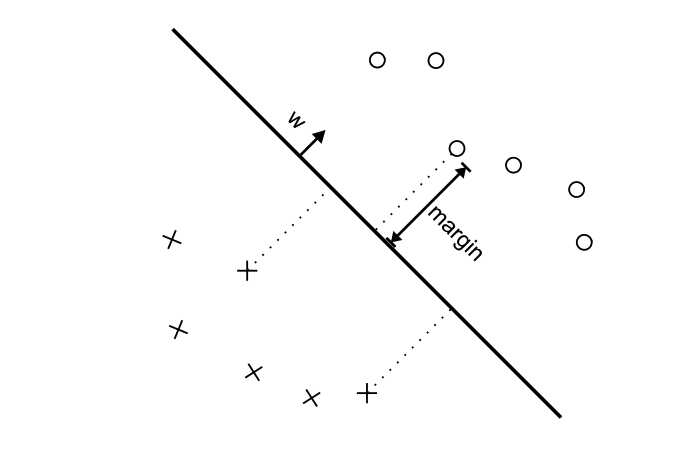
\includegraphics[width=0.5\textwidth]{linear_svm}
  \caption{Двоичная классификация SVM с линейным оператором ядра. $margin$ -- расстояние от
    гиперплоскости до каждого из классов. $w$ -- новый пример, для которого делается предсказание.}\label{linear_svm}
\end{figure}

\subsection{Метод максимальной энтропии}
Следующей рассмотрим классификацию при помощи метода максимальной энтропии~\cite{nigam1999using}. В
случае с разбиением на два класса это использование логистической регрессии для поиска распределения
данных по классам. В отличие от наивного байесовского классификатора этот метод не
предполагает независимости признаков. Это значит, что можно использовать для предсказания признаки
разной природы, например, измерять $n$-граммы\footnote{$n$-буквенные сочетания, например, разбиение
  предложения \textbf{``Мама мыла маму.''} на 3-граммы выглядит так: \textbf{|Мам|а м|ыла| ра|му.|}} и словосочетания в сообщении одновременно.
Суть этого метода в том, что надо выбрать самую
подходящую модель, удовлетворяющую всем естественным ограничениям. Модель описывается формулой:
$$P(c|t,\lambda) = \frac{\exp(\sum_i\lambda_ix_i(c,t))}
{\sum_{c}\exp(\sum_i\lambda_ix_i(c,t))}$$

Здесь $c$ -- метка класса, $t$ -- рассматриваемое сообщение, $x_i(c,t)$ -- совместная
представленность $i$-ого признака в классе $c$ и в примере $t$ , $\lambda$ -- вектор весов для всех
признаков: чем больше вес, тем больше значимость этого признака для классификатора. На этапе обучения
при помощи методов оптимизации вычисляется именно вектор весов признаков. При предсказании класса
для нового примера снова нужно найти такое $c^*$ из множества меток, что рассматриваемая величина $P(c|t,\lambda)$ будет максимальной.

\section{Сравнение работы методов обучения с учителем на данных из Твиттера}

Первичного сравнение проводится на данных, собранных из Твиттера в 2009 году
\cite{go2009twitter}. Здесь мы берём текст в сыром виде, без дополнительной обработки, и передаём
алгоритму. В таблицах \ref{tab:nb}, \ref{tab:svm} и \ref{tab:maxent} представлены результаты работы
наивного байесовского классификатора, классификатора на основе метода опорных векторов и
классификатора по принципу максимальной энтропии соответственно. Алгоритмы обучались на 1,000,000
размеченных примеров и предсказывали результаты для 359 новых.

Чтобы оценить качество классификации, обычно используют $F1-score$ -- гармоническое среднее двух
других: $Precision$ и $Recall$. На языке вероятностей можно определить эти величины следующим образом. $Precision$ -- это
вероятность того, что случайно выбранный твит попал в тот класс, которому он принадлежит
на самом деле. $Recall$ -- это вероятность того, что случайно выбранный твит из класса
при классификации в него и попадёт. Покажем, что значат эти величины более формально.
Пусть зафиксирован класс ``c'' и есть множество всех классифицируемых твитов $\mathcal{T}$,
которое делится на два множества: $\mathcal{T}_c$ -- те, что на самом деле относятся к классу $c$,
и $\mathcal{T}\setminus\mathcal{T}_c$ -- те, у которых стоят другие метки.
По результатам эксперимента определяются следующие величины:
\begin{itemize}
  \item[ ] $TP$ -- количество твитов из множества $\mathcal{T}_с$, которым алгоритм поставил метку $c$;
  \item[ ] $FP$ -- количество твитов из множества $\mathcal{T}\setminus\mathcal{T}_c$, которым алгоритм поставил метку $c$;
  \item[ ] $TN$ -- количество твитов из множества $\mathcal{T}\setminus\mathcal{T}_c$, которым алгоритм поставил метку не $c$;
  \item[ ] $FN$ -- количество твитов из множества $\mathcal{T}_c$, которым алгоритм поставил метку не $c$.
\end{itemize}

Для проверки работы методов использовались реализации из библиотеки SciKit-Learn\footnote{scikit-learn.org}.
В качестве характеристик использовались все слова, встретившиеся в обучающей выборке,
и каждый твит преобразовывлся в вектор из 0 и 1, где 1 ставится
на месте $i$-ого слова, если в сообщении оно присутствует, а 0 -- в противном случае.

\begin{table}[h]
  \begin{minipage}{\textwidth}
    \centering
    \begin{tabular}{|c|c|c|c|c|}
      \hline
      \textbf{Метка класса} & \textbf{Precision} & \textbf{Recall} & \textbf{F1-score} &
      \textbf{Количество} \\ \hline
      -1.0&0.68&0.82&0.74&177\\ \hline
      1.0&0.51&0.79&0.62&182\\ \hline \hline
      avg / total&0.43&0.58&0.49&359\\
      \hline
    \end{tabular}
    \caption{Классификация наивным байесовским классификатором}\label{tab:nb}
  \end{minipage}
\end{table}

\begin{table}[h]
  \begin{minipage}{\textwidth}
    \centering
    \begin{tabular}{|c|c|c|c|c|}
      \hline
      \textbf{Метка класса} & \textbf{Precision} & \textbf{Recall} & \textbf{F1-score} &
      \textbf{Количество} \\ \hline
      -1.0&0.67&0.77&0.72&177\\ \hline
      1.0&0.50&0.81&0.62&182\\ \hline \hline
      avg / total&0.42&0.57&0.48&359\\
      \hline
    \end{tabular}
    \caption{Классификация методом опорных векторов}\label{tab:svm}
  \end{minipage}
\end{table}


\begin{table}
  \begin{minipage}{\textwidth}
    \begin{tabular}{|c|c|c|c|c|}
      \hline
      \textbf{Метка класса} & \textbf{Precision} & \textbf{Recall} & \textbf{F1-score} & \textbf{Количество} \\ \hline
      -1.0&0.72&0.77&0.74&177\\ \hline
      1.0&0.50&0.84&0.62&182\\ \hline \hline
      avg / total&0.44&0.58&0.49&359\\
      \hline
    \end{tabular}
    \caption{Классификация методом максимальной энтропии}\label{tab:maxent}
  \end{minipage}
\end{table}

Как уже было сказано, всего в тестовой выборке было 359 сообщений, из которых 177 были помечены ``+'', а 182 -- ``-''. Каждый